\section{Auswertung}
\label{sec:Auswertung}
\subsection{Bestimmung des magnetischen Moments die Schwingungsdauer}
Die für die Messung erhaltenen Werte befinden sich in Tabelle \ref{tab:schwing}.

\begin{table}[H]
    \centering
    \caption{Messwerte der Schwingung}
      \label{tab:schwing}
    \begin{tabular}{S[table-format=1.2(0)e0] S[table-format=2.1(0)e0] S[table-format=4.3(0)e0] S[table-format=1.3(0)e0] }
        \toprule
        {$I[\si{\ampere}]$} &       {$10\cdot T[\si{\second}]$} &       {$\frac{1}{B}[\si{1\per\tesla}]$} & {$T^2[\si{\second\squared}]$}\\
        \midrule
        0.50   & 19.84  & 1481.481  & 3.936\\
        1.00   & 14.68  &  740.741  & 2.155\\
        1.25   & 14.66  &  592.592  & 2.149\\
        1.50   & 12.12  &  493.827  & 1.468\\
        2.00   & 11.65  &  370.370  & 1.357\\
        2.50   & 10.37  &  296.296  & 1.075\\
        3.00   &  9.50  &  246.913  & 0.902\\
        3.25   &  9.03  &  227.920  & 0.815\\
        3.50   &  8.78  &  211.640  & 0.771\\
        4.00   &  8.25  &  185.185  & 0.681\\
        \bottomrule
    \end{tabular}
\end{table}
$T^2$ wird in Abbildung gegen $\frac{1}{B}$ aufgetragen.
Durch dieses Werte wird eine Gerade mittels linearer Regression aufgetragen.
\begin{figure}[H]
  \centering
  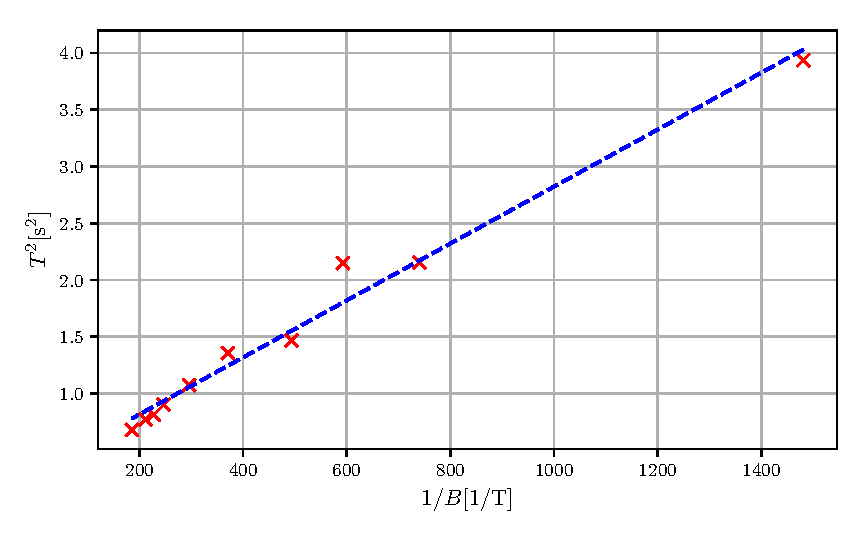
\includegraphics{schwing.pdf}
  \caption{.}
  \label{fig:schwing}
\end{figure}
Daraus folgt eine Steigung von $m=0.00251 \pm 0.00012$ für die lineare Ausgleichsgerade.
Das magnetische Moment lässt sich dann nach Formel\eqref{eq:schwing} berechnen:
\begin{equation}
  \mu_{Dipol}= \frac{\pi^2 \cdot J_{Kugel}}{m}=(0.59)\si{\ampere\meter\squared}
\end{equation}
\subsection{Bestimmung des magnetischen Moments über Präzession}
Da es schwierig war eine konstante Frequenz einzustellen sind die für die Messung angegebenen Werte gemittelt.
Diese Werte befinden sich in Tabelle \ref{tab:praes}.
\begin{table}[H]
    \centering
      \label{tab:praes}
    \sisetup{table-format=3.2(4)}
    \caption{Messwerte der Präzession}
    \begin{tabular}{S S S S}
        \toprule
        {$B\cdot 10^-3[\si{\tesla}]$} &       {$\bar{T}[\si{\second}]$} &      {$\bar{\nu}[\si{\hertz}]$}\\
        \midrule
        0.67   & 29.00\pm 0.41  &  6.97\pm 0.17\\
        1.35   & 18.59\pm 0.84  &  7.56\pm 0.38\\
        2.00   & 10.99\pm 0.59  &  6.60\pm 0.43\\
        2.70   &  8.47\pm 0.16  &  6.53\pm 0.09\\
        3.30   &  6.96\pm 0.25  &  6.70\pm 0.38\\
        3.70   &  6.41\pm 0.17  &  6.93\pm 0.33\\
        4.00   &  6.31\pm 0.26  &  6.36\pm 0.29\\
        4.70   &  5.49\pm 0.34  &  7.36\pm 0.44\\
        5.00   &  4.51\pm 0.21  &  6.60\pm 0.49\\
        5.40   &  4.60\pm 0.18  &  6.90\pm 0.58\\
        \bottomrule
    \end{tabular}
\end{table}
In der Abbildung \ref{fig:praes} wurde die reziproke Periodendauer gegen die Magnetfeldstärke aufgetragen.
Zusätzlich wurde eine Regressionsgerade aufgetragen.
\begin{figure}[H]
  \centering
  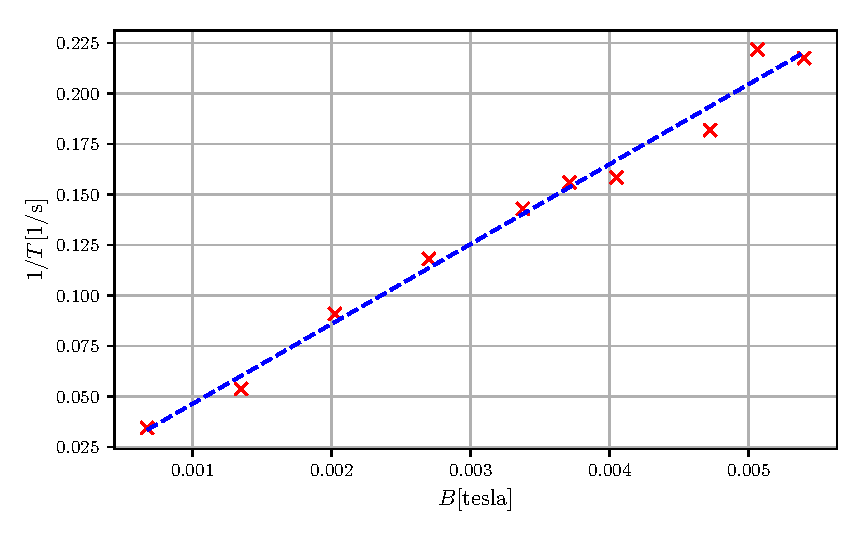
\includegraphics{praes.pdf}
  \caption{.}
  \label{fig:praes}
\end{figure}
Für die Steigung der Geraden ergibt sich ein Wert von $m=(39.5 \pm 1.7)$.
Damit lässt sich das magnetische Moment nach Gleichung\eqref{eq:praes} berechnen:
\begin{equation}
     \mu_\text{Dipol}=m\cdot 2\pi \cdot L_{Kugel} .
\end{equation}
